\documentclass[xcolor=dvipsnames]{beamer}
\usepackage[T1]{fontenc}
\usepackage[utf8]{inputenc}
\usepackage[english,slovak]{babel}

\usepackage{amsmath}
\usepackage{amsthm}
\usetheme{Pittsburgh}
\useoutertheme{shadow}

\usepackage{graphicx}
\usepackage{caption}
\usepackage{subcaption}

\usepackage[]{algorithm2e}
\usepackage{listings}
 \setbeamercovered{transparent}
 \usepackage{cuted}
\usepackage[export]{adjustbox}
\usepackage{mathtools}

\usepackage{lipsum}
\usepackage{verbatim}
\usepackage{transparent}
\usepackage{framed}
\usepackage{xcolor}

\usepackage{multirow}
\usepackage{colortbl}

\newcommand\Wider[2][3em]{%
\makebox[\linewidth][c]{%
  \begin{minipage}{\dimexpr\textwidth+#1\relax}
  \raggedright#2
  \end{minipage}%
  }%
}




\iftrue

\usetheme{Warsaw}

\setbeamercolor{normal text}{fg=white,bg=black!90}
\setbeamercolor{structure}{fg=white}

\setbeamercolor{alerted text}{fg=red!85!black}

\setbeamercolor{item projected}{use=item,fg=black,bg=item.fg!35}

\setbeamercolor*{palette primary}{use=structure,fg=structure.fg}
\setbeamercolor*{palette secondary}{use=structure,fg=structure.fg!95!black}
\setbeamercolor*{palette tertiary}{use=structure,fg=structure.fg!90!black}
\setbeamercolor*{palette quaternary}{use=structure,fg=structure.fg!95!black,bg=black!80}

\setbeamercolor*{framesubtitle}{fg=white}

\setbeamercolor*{block title}{parent=structure,bg=black!60}
\setbeamercolor*{block body}{fg=black,bg=black!10}
\setbeamercolor*{block title alerted}{parent=alerted text,bg=black!15}
\setbeamercolor*{block title example}{parent=example text,bg=black!15}

\fi



%-------------------------------------------------------------------------------------
\title{\color{white} \bf AlphaGo, AlphaZero, AlphaStar - Google DeepMind}
\author{\color{white} Michal CHOVANEC, PhD}


%\setbeamertemplate{footline}[frame number]{}
\setbeamertemplate{navigation symbols}{}


\date[EURP]{}
\begin{document}

{
    \usebackgroundtemplate
    {
        \vbox to \paperheight{\vfil\hbox to \paperwidth{\hfil

        {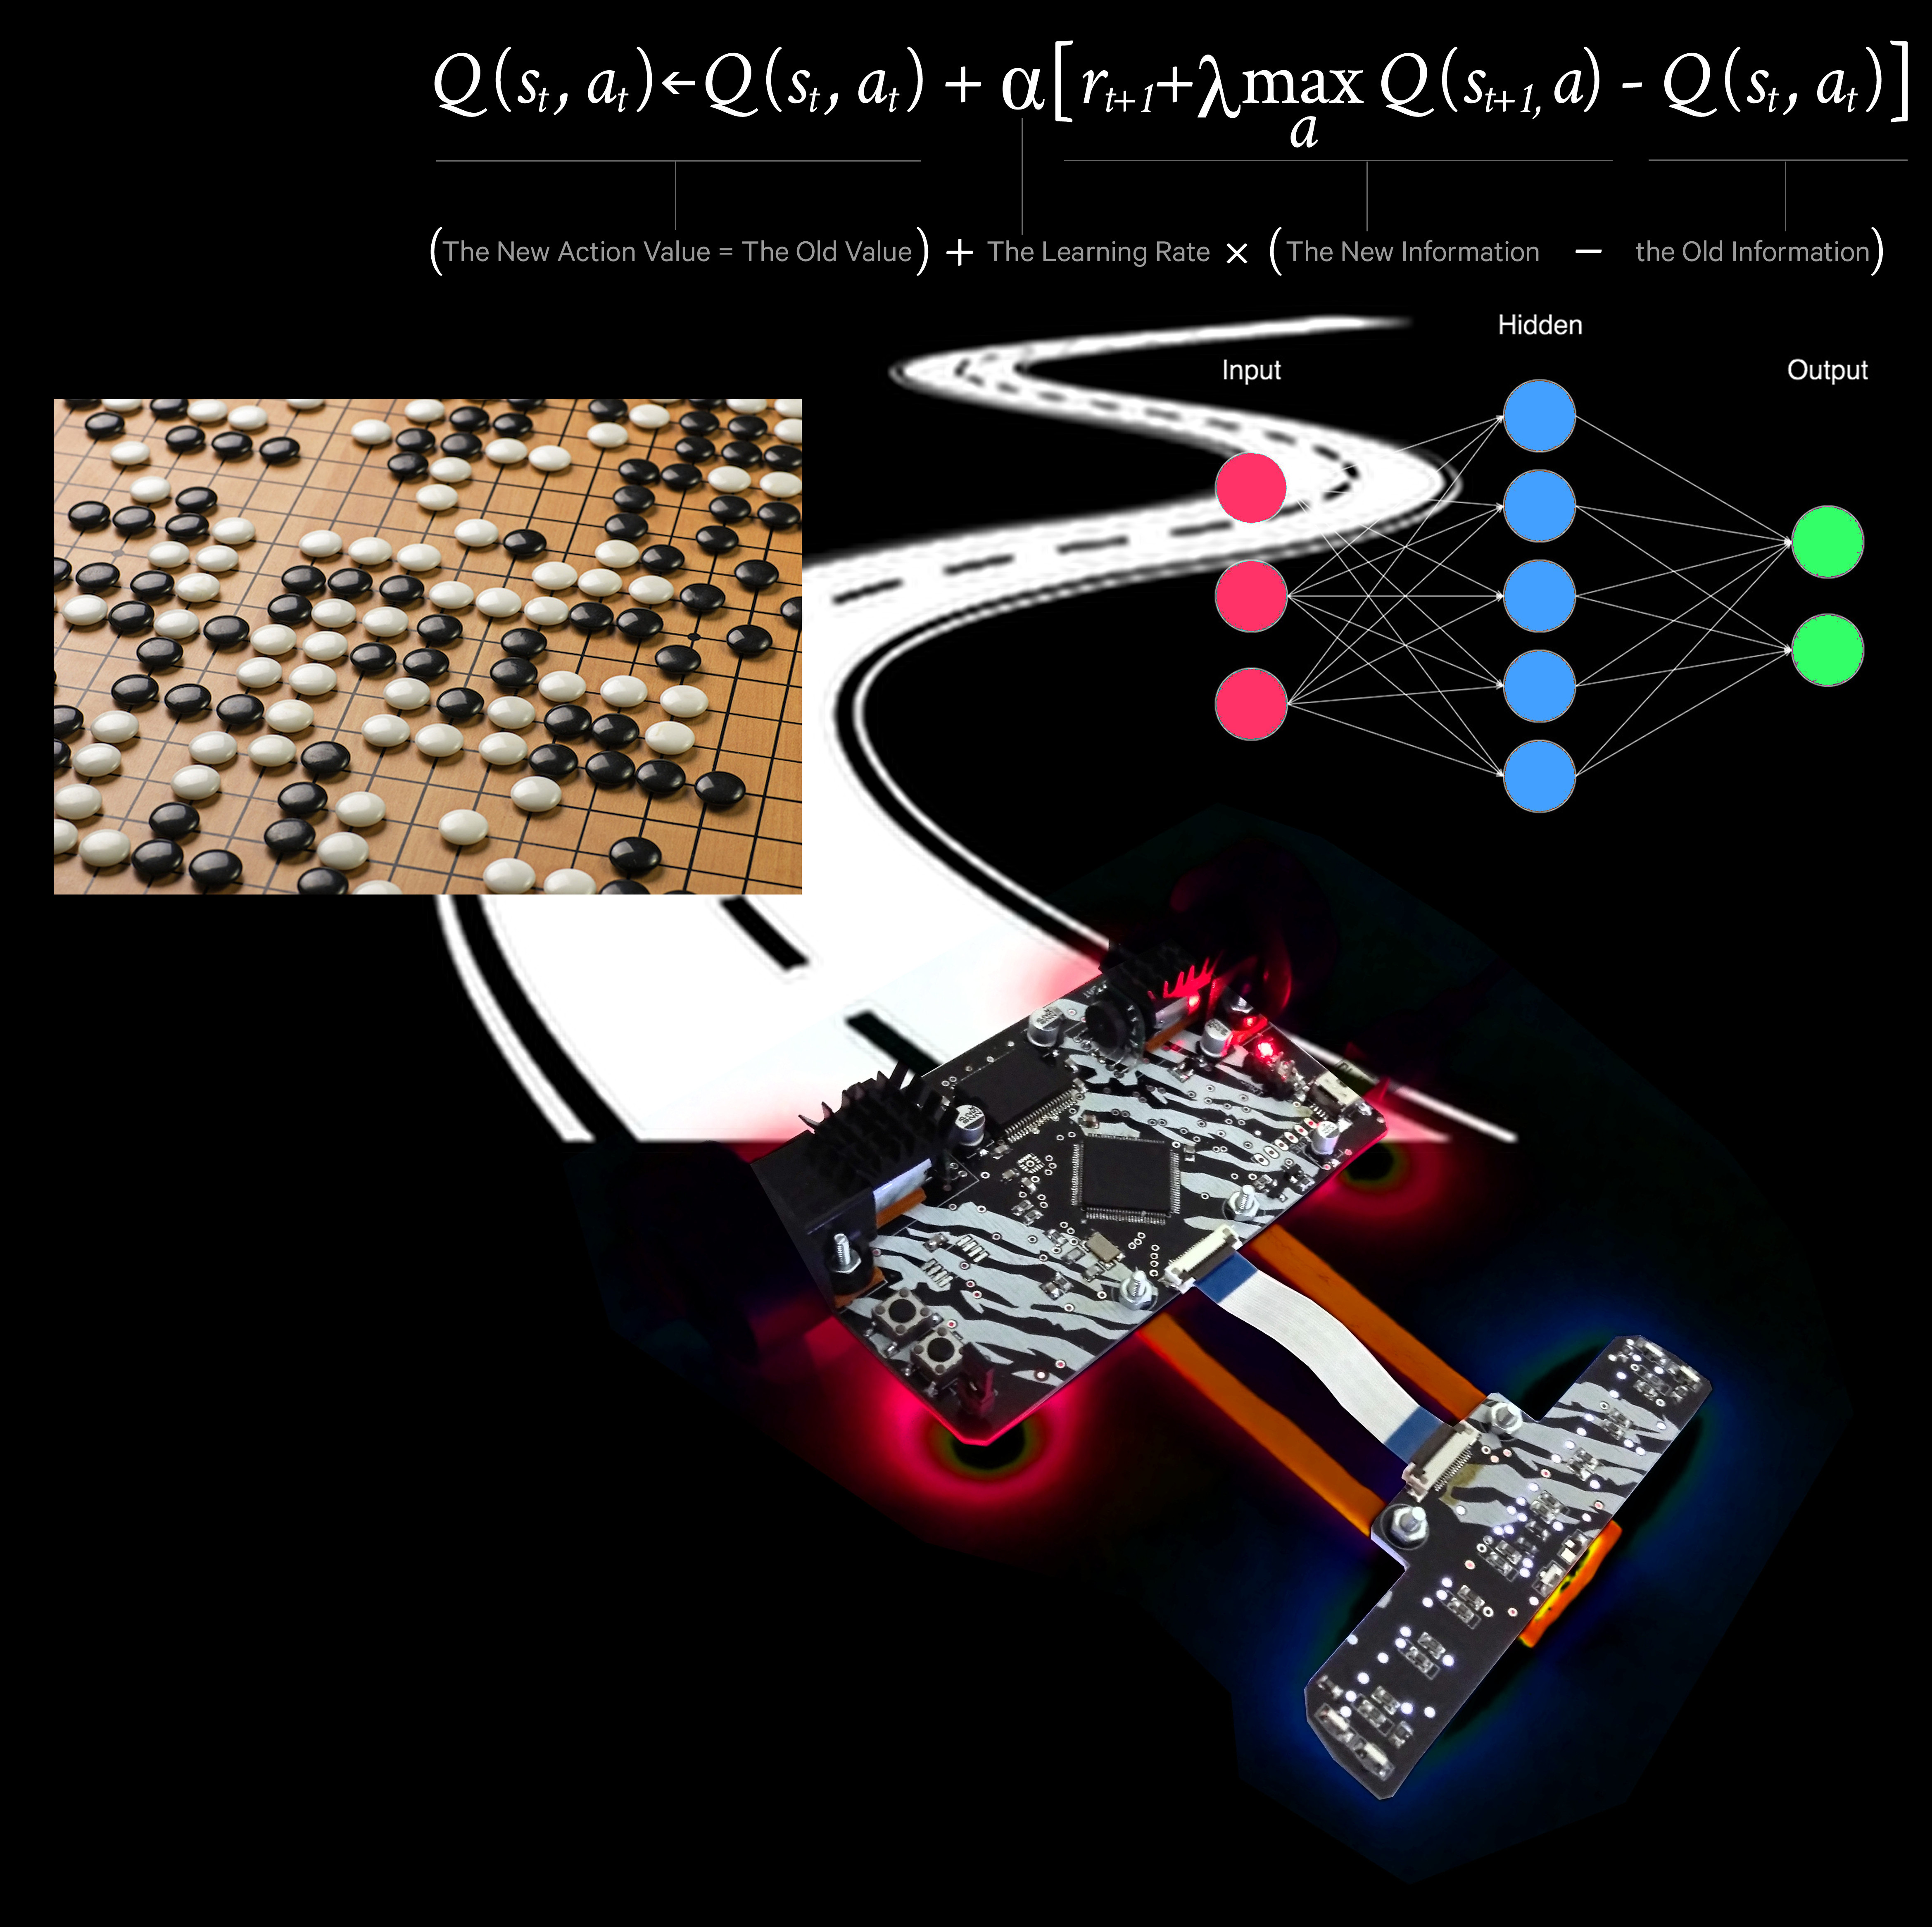
\includegraphics[width=5.05in]{../../pictures/rl_square.jpg}}

        \hfil}\vfil}
    }
    \begin{frame}

    %\titlepage


    \centering
     \colorbox{black}
     {
        \begin{minipage}{12cm}
           {\LARGE \color{white} \bf AlphaGo, AlphaZero, AlphaStar \\- Google DeepMind} \\
           {\LARGE \color{white} Michal CHOVANEC, PhD} \\
       \end{minipage}
     }


    \end{frame}
}



\begin{frame}{\bf End of Deep learning middle age}

\begin{itemize}
  \item {\color{red} \bf GO} : AlphaGO vs Lee Sedol, 4 - 1, 9th .. 15th Match 2016
            {\tiny \url{https://deepmind.com/documents/119/agz\_unformatted\_nature.pdf}}
  \item {\color{red} \bf Chess} : AlphaZero vs StockFish,  W290 - D886 - L24, December 2017
            {\tiny \url{https://arxiv.org/pdf/1712.01815.pdf}}
  \item {\color{red} \bf StarCraft} : AlphaStar vs MaNa, 5-0, 19th December 2019
            {\tiny \url{https://deepmind.com/blog/alphastar-mastering-real-time-strategy-game-starcraft-ii/}}
\end{itemize}

\end{frame}


\begin{frame}{\bf GO}

\begin{figure}[!htb]
  \centering
  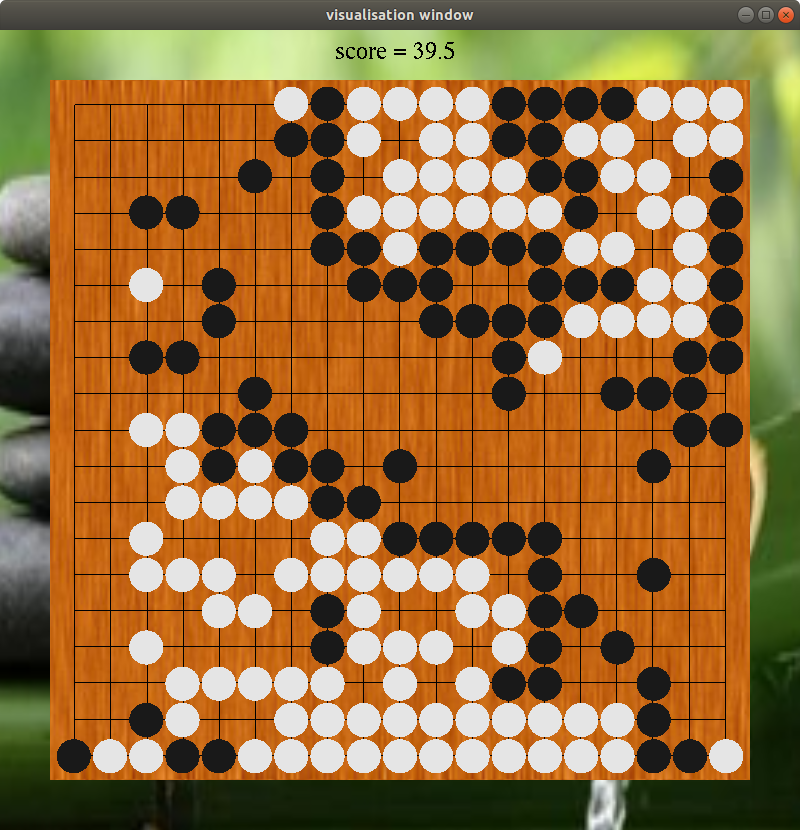
\includegraphics[scale=0.2]{../../pictures/go_board.png}
\end{figure}

\end{frame}


\begin{frame}{\bf Game complexity}

\begin{itemize}
    \item $10^{170}$ legal positions, chess $10^{120}$, atoms in universe $10^{80}$
    \item 200 moves per position (average) (20 in chess)
    \item best (old) progamms using MonteCarlo tree search \\
        - can't beat profesional Dan players
\end{itemize}

\begin{columns}
\begin{column}{0.5\textwidth}

\begin{figure}[!htb]
  \centering
  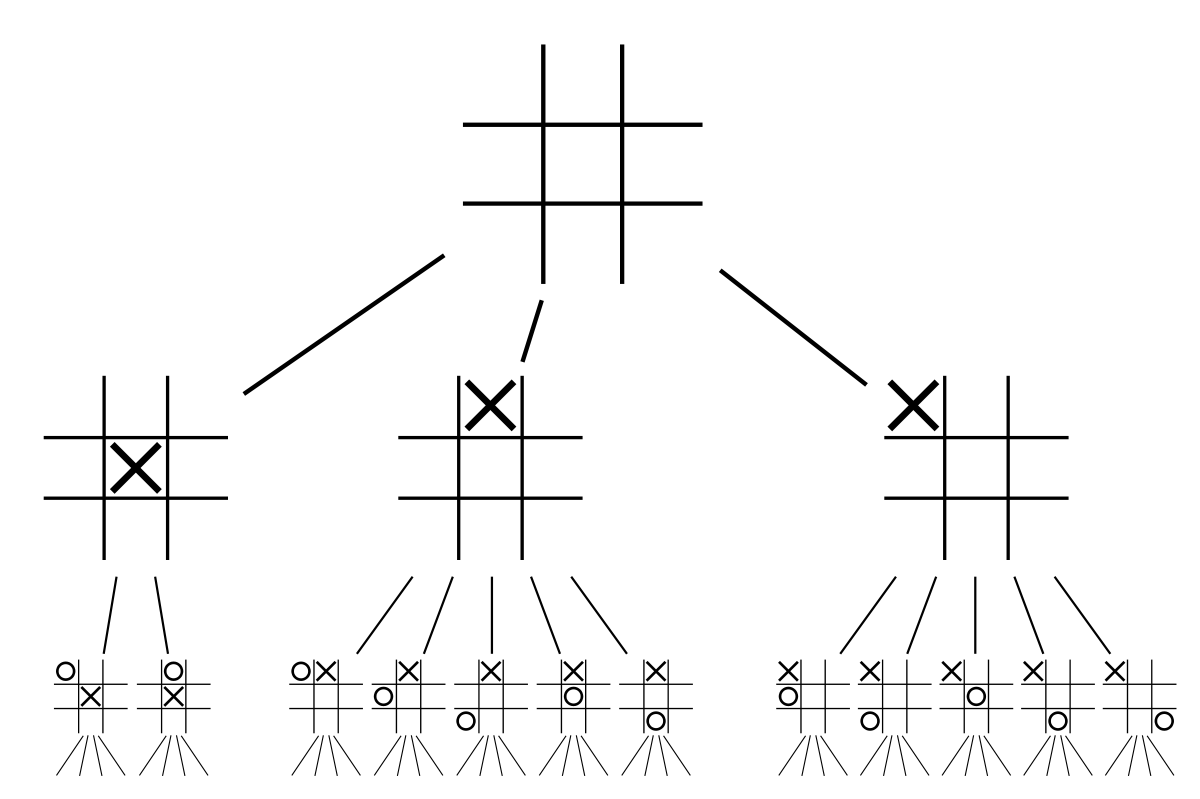
\includegraphics[scale=0.1]{../../pictures/tic_tac.png}
\end{figure}

\end{column}
\begin{column}{0.5\textwidth}  %%<--- here


\begin{figure}[!htb]
  \centering
  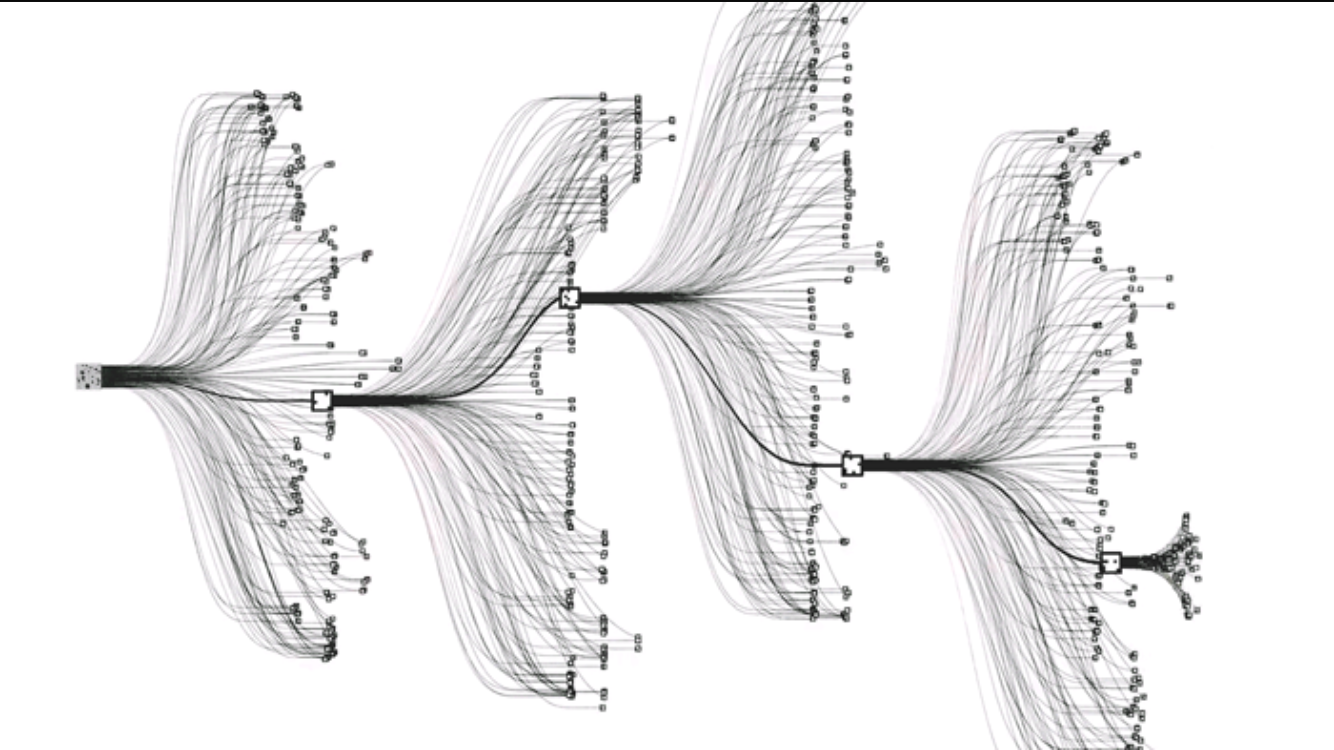
\includegraphics[scale=0.1]{../../pictures/go_tree.png}
\end{figure}

\end{column}
\end{columns}


\end{frame}


\begin{frame}{\bf AlphaGo architecture}


\begin{itemize}
    \item Two neural networks \\
    - Policy network, Value network
    \item Policy network - give probabilities of good / wrong moves
    \item Value network - give probability of winning / loosing
\end{itemize}

\begin{figure}[!htb]
  \centering
  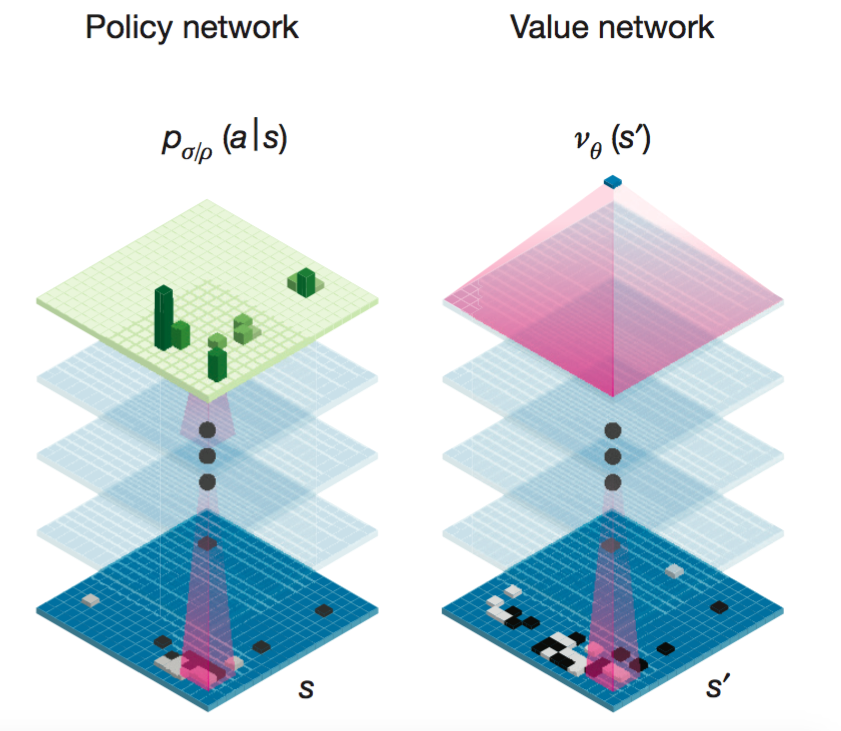
\includegraphics[scale=0.2]{../../pictures/alpha_go_architecture.png}
\end{figure}

\end{frame}


\begin{frame}{\bf AlphaGo architecture}


\begin{itemize}
    \item Two neural networks \\
    - Policy network, Value network
    \item Policy network - give probabilities of good / wrong moves
    \item Value network - give probability of winning / loosing
\end{itemize}

\begin{columns}
\begin{column}{0.5\textwidth}

\begin{figure}[!htb]
  \centering
  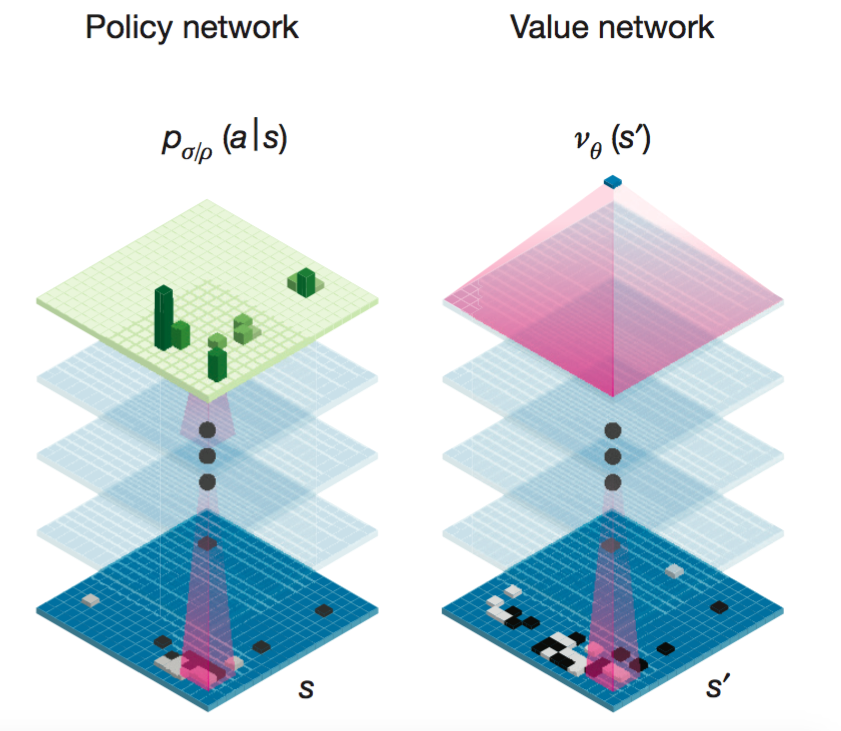
\includegraphics[scale=0.2]{../../pictures/alpha_go_architecture.png}
\end{figure}

\end{column}
\begin{column}{0.5\textwidth}  %%<--- here

\begin{itemize}
    \item input \\
        {\footnotesize
        - stones positions with feature planes \\
        - black, white, legal positions \\
        - actual player on move \\
        - ... \\
        Tensor $19x19xfeature\_planes$
        }
    \item output \\
        - Policy network 19x19 probabilities
        - Value network 2 black and white win probabilities
\end{itemize}

\end{column}
\end{columns}

\end{frame}

\begin{frame}{\bf Game 4, Lee Sedol wins}

Move 78 - "divine move" Gu Li, 15\% win drop

\begin{figure}[!htb]
  \centering
  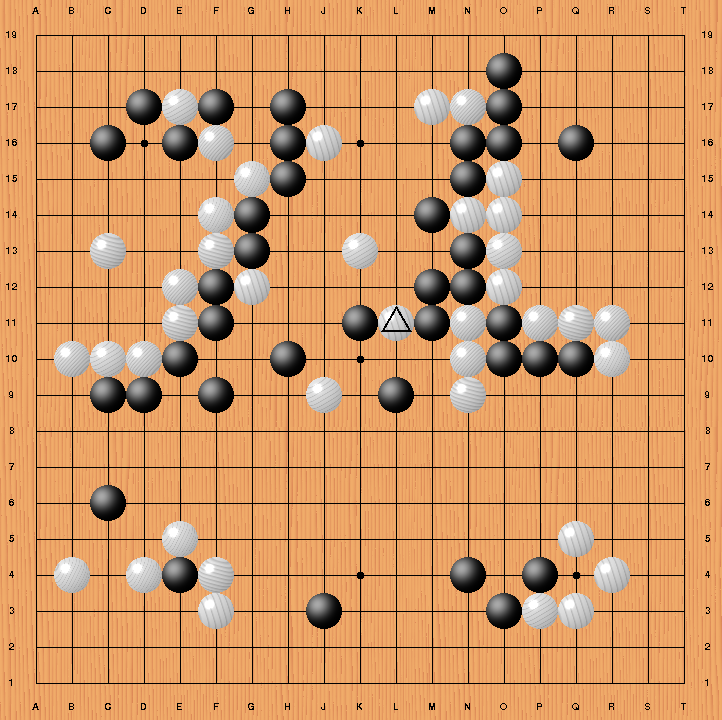
\includegraphics[scale=0.2]{../../pictures/alpha_go_game_4.png}
\end{figure}

\end{frame}




\begin{frame}{\bf My GO net}


  \begin{columns}
  \begin{column}{0.5\textwidth}

    \begin{figure}[!htb]
      \centering
      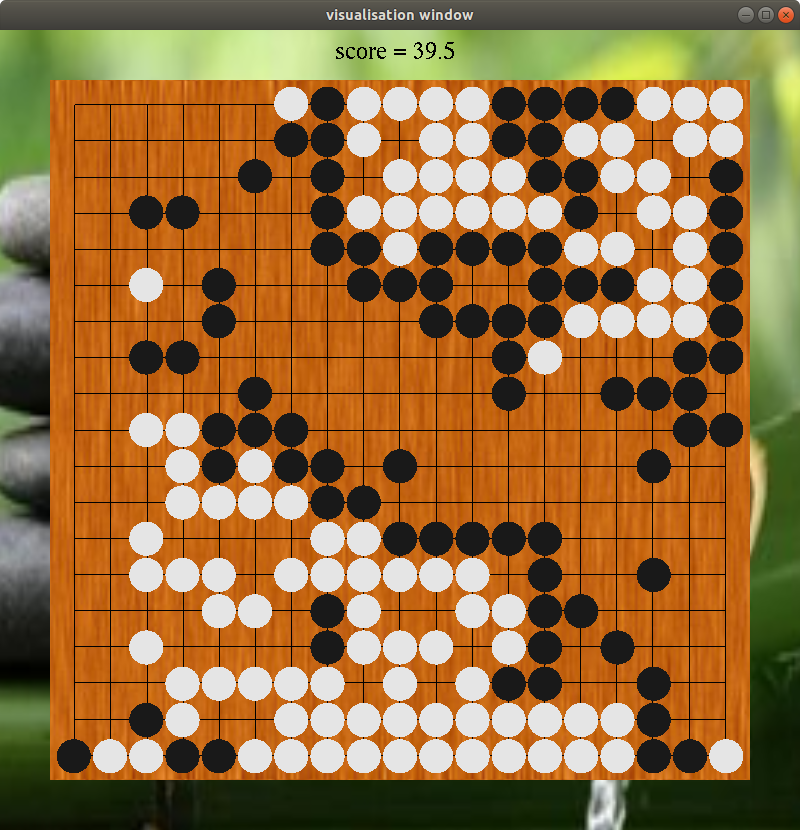
\includegraphics[scale=0.18]{../../pictures/go_board.png}
    \end{figure}


  \end{column}
  \begin{column}{0.5\textwidth}  %%<--- here

    \scriptsize
    {
      \begin{itemize}
        \item {\bf supervised training} - train game using Masters games
        \item {\bf reinforcement learning} - let play two networks against each other
      \end{itemize}
    }
  \end{column}
  \end{columns}

\end{frame}

\begin{frame}{\bf Network architecture}
we need to go much deeper for GO
\begin{itemize}
  \item {\bf 27 convolutional layers} \\ 3 blocks with 8 dense conv + 1 conv layer
  \item {\bf input} \\ 4 matrices $19x19$: black stones, white stones, empty fields, active player
  \item {\bf output} \\ recommended moves 19x19 + 1 for pass = 362 outputs

\end{itemize}

  \begin{figure}[!htb]
    \centering
    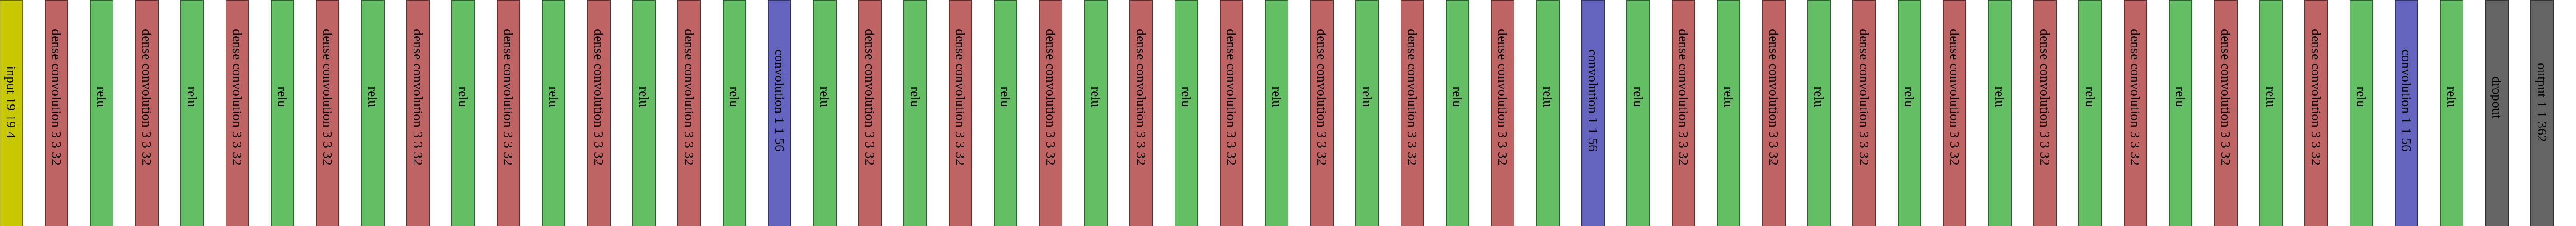
\includegraphics[scale=0.07]{../../pictures/go_cnn.png}
  \end{figure}

\end{frame}

\begin{frame}{\bf Network architecture}

{\fontsize{8}{6}\selectfont

\begin{table}[]
\begin{tabular}{|c|l|l|}
\hline
\textbf{layer} & \multicolumn{1}{c|}{\textbf{net 3}}       & \multicolumn{1}{c|}{\textbf{net 5}}       \\ \hline
0              & \cellcolor[HTML]{FD6864}dense conv 5x5x32 & \cellcolor[HTML]{FD6864}dense conv 3x3x32 \\ \hline
1              & \cellcolor[HTML]{FD6864}dense conv 5x5x32 & \cellcolor[HTML]{FD6864}dense conv 3x3x32 \\ \hline
2              & \cellcolor[HTML]{FD6864}dense conv 5x5x32 & \cellcolor[HTML]{FD6864}dense conv 3x3x32 \\ \hline
3              & \cellcolor[HTML]{FD6864}dense conv 5x5x32 & \cellcolor[HTML]{FD6864}dense conv 3x3x32 \\ \hline
4              & \cellcolor[HTML]{38FFF8}conv 1x1x32       & \cellcolor[HTML]{FD6864}dense conv 3x3x32 \\ \hline
5              & \cellcolor[HTML]{FD6864}dense conv 5x5x32 & \cellcolor[HTML]{FD6864}dense conv 3x3x32 \\ \hline
6              & \cellcolor[HTML]{FD6864}dense conv 5x5x32 & \cellcolor[HTML]{FD6864}dense conv 3x3x32 \\ \hline
7              & \cellcolor[HTML]{FD6864}dense conv 5x5x32 & \cellcolor[HTML]{FD6864}dense conv 3x3x32 \\ \hline
8              & \cellcolor[HTML]{FD6864}dense conv 5x5x32 & \cellcolor[HTML]{38FFF8}conv 1x1x56       \\ \hline
9              & \cellcolor[HTML]{38FFF8}conv 1x1x32       & \cellcolor[HTML]{FD6864}dense conv 3x3x32 \\ \hline
10             & \cellcolor[HTML]{FD6864}dense conv 5x5x32 & \cellcolor[HTML]{FD6864}dense conv 3x3x32 \\ \hline
11             & \cellcolor[HTML]{FD6864}dense conv 5x5x32 & \cellcolor[HTML]{FD6864}dense conv 3x3x32 \\ \hline
12             & \cellcolor[HTML]{FD6864}dense conv 5x5x32 & \cellcolor[HTML]{FD6864}dense conv 3x3x32 \\ \hline
13             & \cellcolor[HTML]{FD6864}dense conv 5x5x32 & \cellcolor[HTML]{FD6864}dense conv 3x3x32 \\ \hline
14             & \cellcolor[HTML]{38FFF8}conv 1x1x32       & \cellcolor[HTML]{FD6864}dense conv 3x3x32 \\ \hline
15             & \cellcolor[HTML]{FD6864}dense conv 5x5x32 & \cellcolor[HTML]{FD6864}dense conv 3x3x32 \\ \hline
16             & \cellcolor[HTML]{FD6864}dense conv 5x5x32 & \cellcolor[HTML]{FD6864}dense conv 3x3x32 \\ \hline
17             & \cellcolor[HTML]{FD6864}dense conv 5x5x32 & \cellcolor[HTML]{38FFF8}conv 1x1x56       \\ \hline
18             & \cellcolor[HTML]{FD6864}dense conv 5x5x32 & \cellcolor[HTML]{FD6864}dense conv 3x3x32 \\ \hline
19             & \cellcolor[HTML]{38FFF8}conv 5x5x64       & \cellcolor[HTML]{FD6864}dense conv 3x3x32 \\ \hline
20             & \cellcolor[HTML]{67FD9A}fc 362            & \cellcolor[HTML]{FD6864}dense conv 3x3x32 \\ \hline
21             &                                           & \cellcolor[HTML]{FD6864}dense conv 3x3x32 \\ \hline
22             &                                           & \cellcolor[HTML]{FD6864}dense conv 3x3x32 \\ \hline
23             &                                           & \cellcolor[HTML]{FD6864}dense conv 3x3x32 \\ \hline
24             &                                           & \cellcolor[HTML]{FD6864}dense conv 3x3x32 \\ \hline
25             &                                           & \cellcolor[HTML]{FD6864}dense conv 3x3x32 \\ \hline
26             &                                           & \cellcolor[HTML]{38FFF8}conv 1x1x64       \\ \hline
27             &                                           & \cellcolor[HTML]{67FD9A}fc 362            \\ \hline
\end{tabular}
\end{table}
}


\end{frame}


\begin{frame}{\bf Supervised results}

\begin{figure}[!htb]
  \centering
  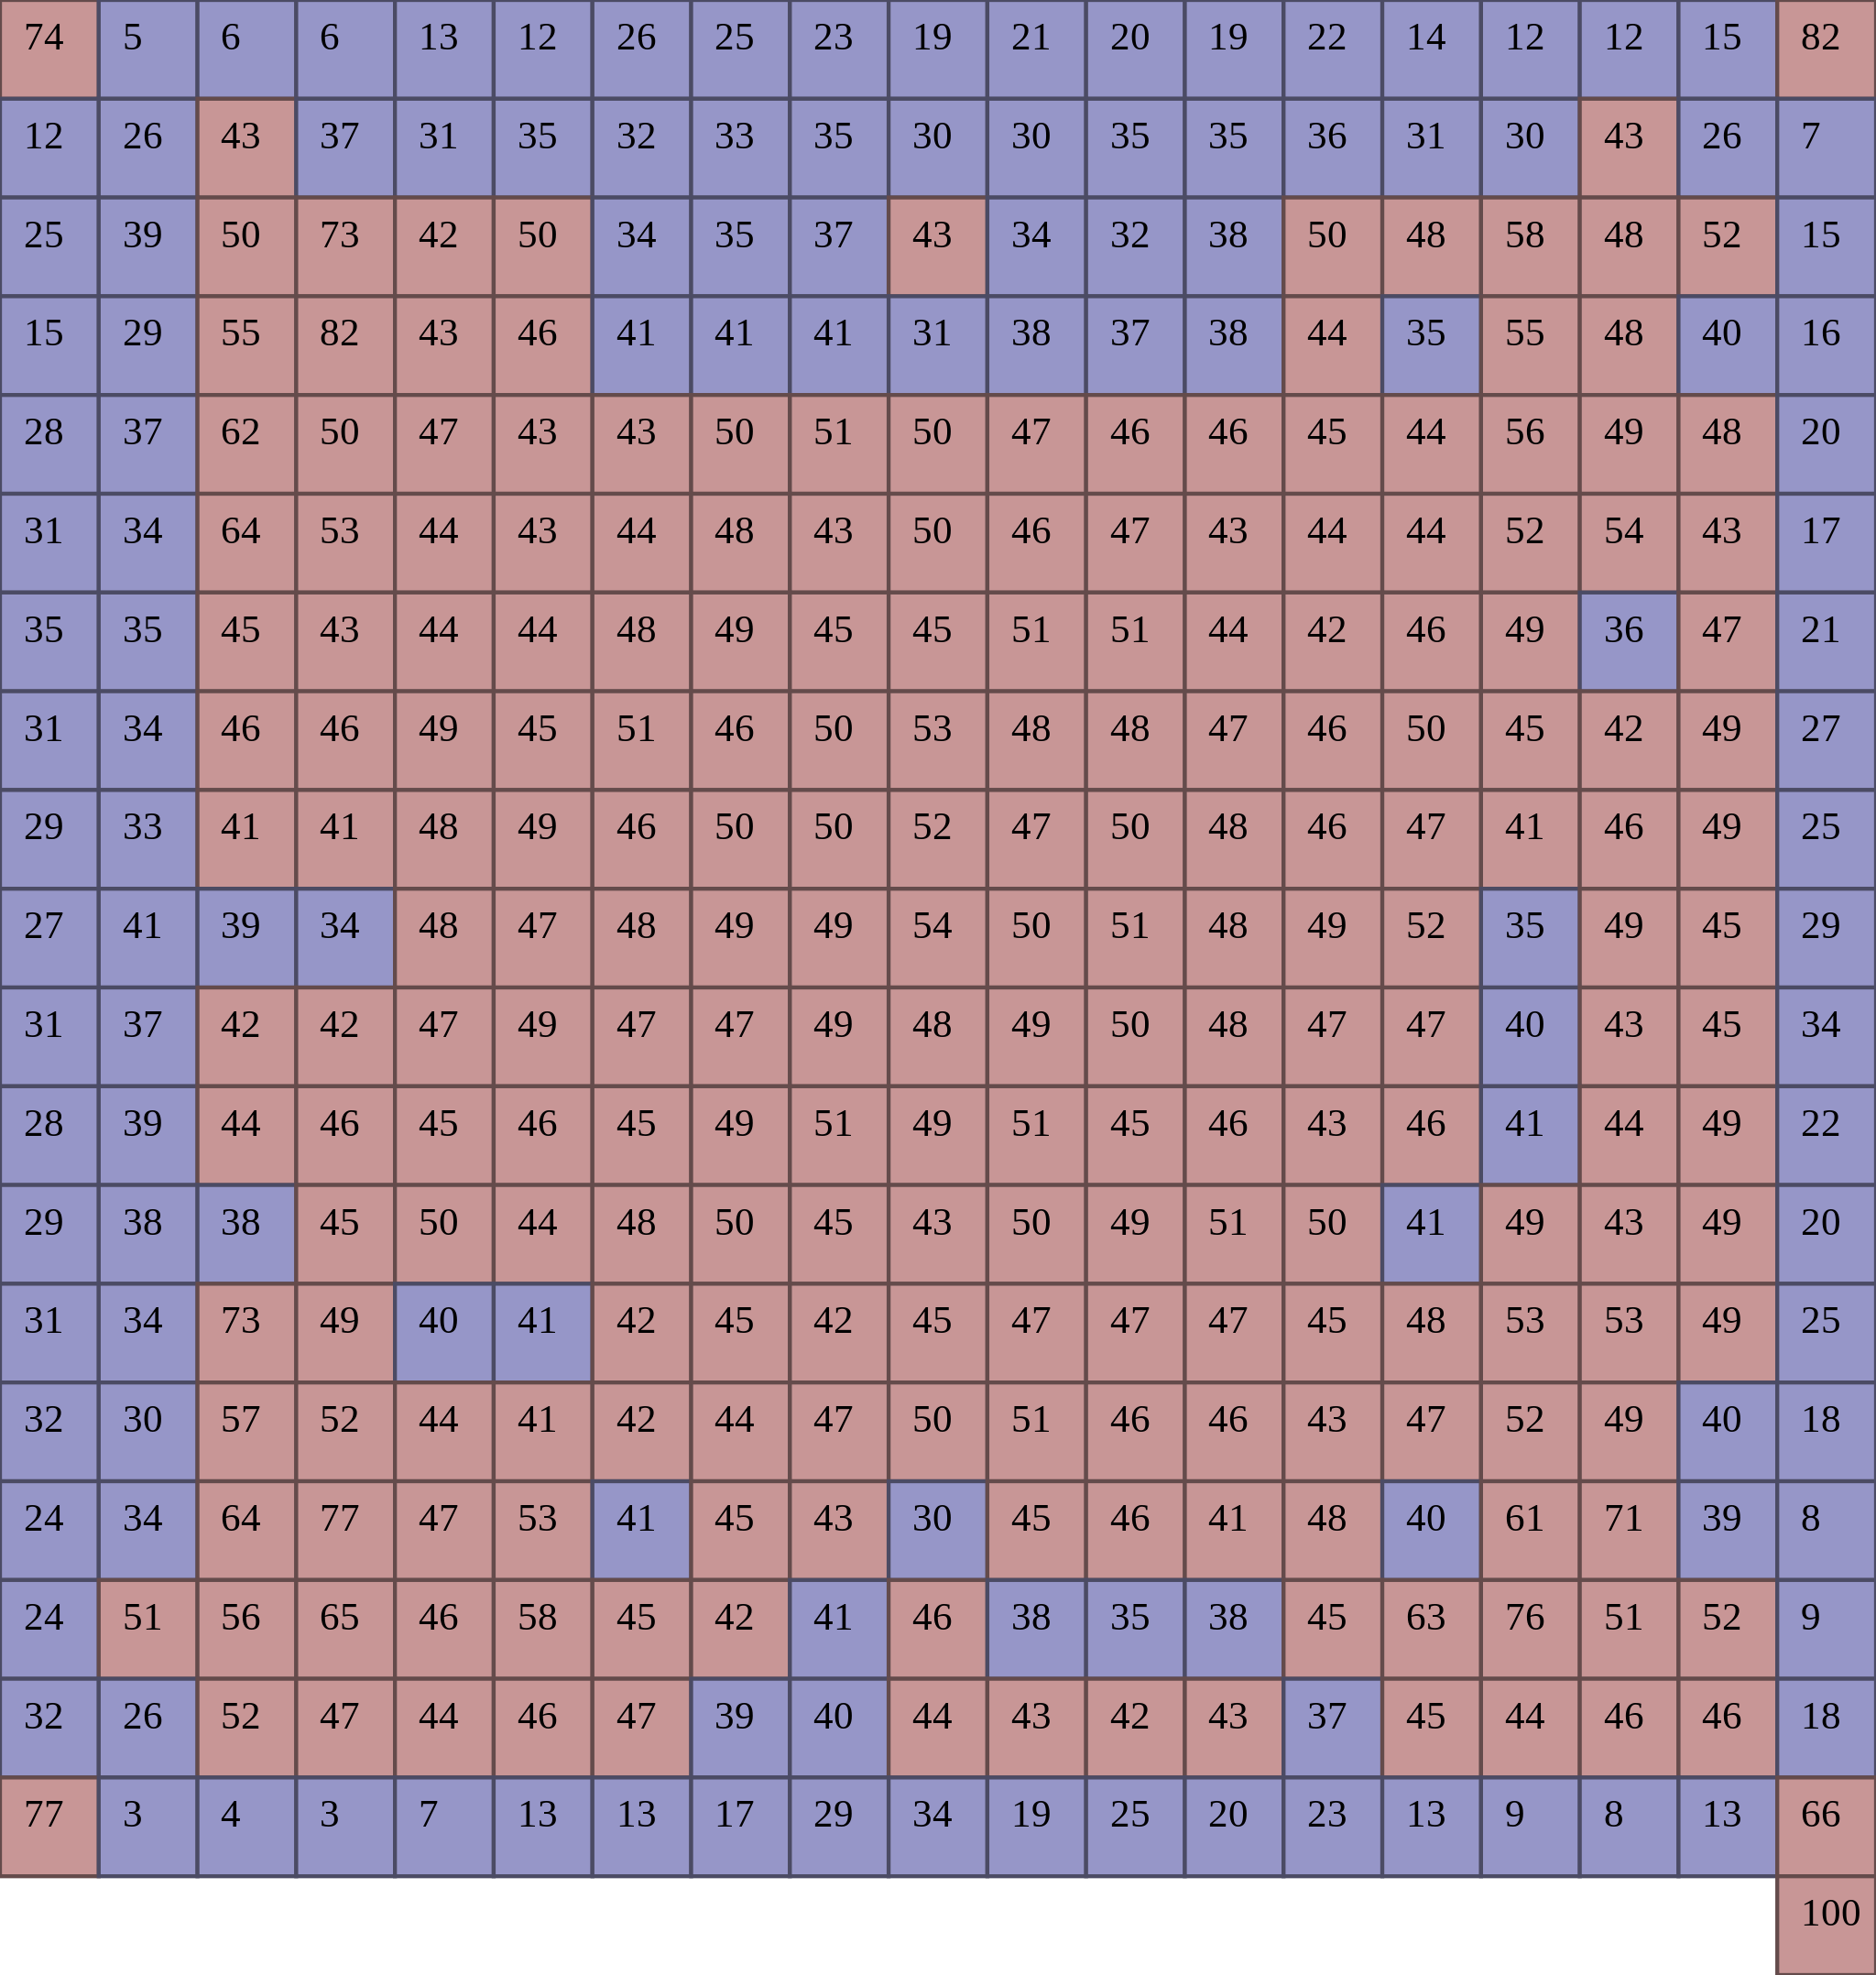
\includegraphics[scale=0.22]{../../pictures/moves_success_rate_testing_top5.png}
\end{figure}


\end{frame}



\begin{frame}{\bf Q\&A}

\begin{figure}
  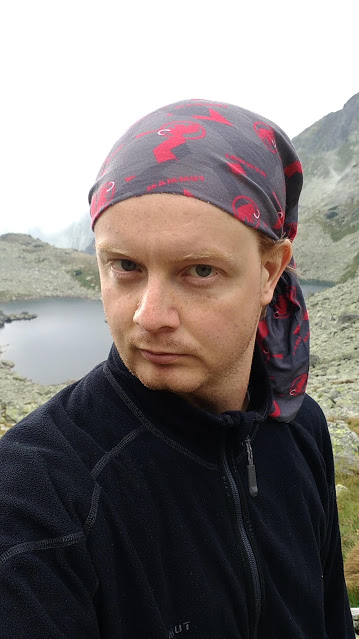
\includegraphics[scale=0.25]{../../pictures/me.jpg}
\end{figure}

\centering {
michal chovanec (michal.nand@gmail.com)
\url{www.youtube.com/channel/UCzVvP2ou8v3afNiVrPAHQGg}
}

\centering {
github
\url{https://github.com/michalnand}
}

\end{frame}


\end{document}
